\chapter{Réduction des endomorphismes}
\labch{reduction_des_endomorphismes}

{\Large Diagonalisation \sidenote[][-2mm]{Le texte suivant est extrait de \cite{oraux_x_ens_2} p. 169.}} \\

\textsl{On doit à Camille \textsc{Jordan} de nombreux résultats sur la réduction des endomorphismes qu'il découvre notamment à travers l'étude des groupes. Dépassant la notion des groupes de permutations pour en atteindre une plus abstraite, il s'intéresse à la classification des groupes finis à travers leurs représentations linéaires, autrement dit les morphismes entre un groupe fini $G$ et le groupe linéaire $\Gl (E)$ d'un espace vectoriel $E$. Il va même jusqu'à donner le description des classes de similitudes à l'aide des formes dites de \textsc{Jordan}.}\\
\textsl{Le problème fondamental de la réduction est bien celui de caractériser les classes de similitude de l'algèbre $\Endo(E)$ où $E$ est un $\K$-espace vectoriel de dimension finie ou, ce qui revient au même, les classes de similitudes de l'agèbre $\M_n(\K)$. La recherche d'une matrice la plus simple possible pour représenter un endomorphisme donné vise de multiples buts: calculer les puissances successives de cet endomorphisme, son commutant, résoudre des systèmes différentiels linéaires... Une idée naturelle pour essayer de "réduire" l'étude d'un endomorphisme $u$ donné à des choses plus simples consiste à essayer de décomposer l'espace vectoriel $E$ en une somme directe de sous-espaces non triviaux stables par $u$. Cela n'est évidemment pas toujours possible. Les sous-espaces stables les plus simples sont ceux sur lesquels $u$ coïncide avec une homothétie. On est ainsi naturellement amené à la notion de valeur propre. Si $\lambda$ est un scalaire, on s'intéresse donc au sous-espace $E_\lambda = \Ker(u - \lambda \Id_E)$ appelé sous-espace propre pour la valeur propre $\lambda$ lorsque celui-ci n'est pas nul. Le théorème de décomposition des noyaux nous assure que les différents sous-espaces propres d'un endomorphisme sont en somme directe. Le cas où la somme remplit tout l'espace $E$ mène à la notion d'endomorphisme diagonalisable: un tel endomorphisme peut être représenté par une matrice diagonale (il suffit de prendre une base formée de vecteurs propres). Pour les endomorphismes diagonalisables il est alors très facile de répondre à la question initiale de savoir quand ils sont semblables: il faut et suffit qu'ils aient les mêmes valeurs propres et que les espaces propres associés aient la même dimension. Il est aussi facile, en se ramenant à une matrice diagonale, de calculer les puissances d'un tel endomorphisme, son exponentielle (si on travaille sur un sous-corps de $\C$), son commutant...} \\

Soit $E$ un espace vectoriel de dimension finie. Un endomorphisme $u$ de $E$ est trigonalisable si et seulement s'il existe un drapeau total de $E$ stable par $u$. 

\begin{marginfigure}[-19cm]
    \includegraphics{images/camille_jordan.jpg}
    \caption{Camille \textsc{Jordan}}
\end{marginfigure}

\section{Matrices à diagonale dominante}
\begin{defi}
    Soit $A = (a_{i,j}) \in \M_n(\K)$. On dit que $A$ est 
    \begin{itemize}
        \item à \emph{diagonale dominante} si
        $$\forall i \in \llbracket 1, n \rrbracket,\ |a_{i,i}| \geqslant \sum_{k \not = i} |a_{i,k}|,$$
        \item à \emph{diagonale fortement dominante} si de plus l'inégalité est stricte pour une valeur de $i$ au moins,
        \item à \emph{diagonale strictement dominante} si l'inégalité est stricte pour tout $i$. 
    \end{itemize}
\end{defi}

\begin{lemme} \label{lemme_hadamard}
    Toute matrice à diagonale strictement dominante (DSD) est inversible.
\end{lemme}

\marginnote[2cm]{
    \begin{methode}
        $$\left |x_{i_0} \right | \defeq \max_{1 \leqslant i \leqslant n} |x_i|$$
    \end{methode}
}

\begin{preuve}
    Soit $X = \Trsp{(x_1 \cdots x_n)} \in \Ker(A)$. \\
    On pose $\displaystyle \left |x_{i_0} \right| \defeq \max_{1 \leqslant i \leqslant n} |x_i|$. La ligne $i_0$ de la relation $AX = 0$ donne
    $$\sum_{j=1}^n a_{i_0,j}x_j = 0$$
    soit
    $$-a_{i_0, i_0} x_{i_0} = \sum_{j \not = i_0} a_{i_0,j} x_j$$
    d'où, d'après l'inégalité triangulaire,
    $$|a_{i_0, i_0}| |x_{i_0}| \leqslant \sum_{j \not = i_0} |a_{i_0,j}| |x_j| \leqslant |x_{i_0}| \sum_{j \not = i_0} |a_{i_0, j}|.$$
    Comme $|a_{i_0, i_0}| > \sum\limits_{j \not = i_0} |a_{i_0, j}|$ par définition de $A$, on en déduit que
    $|x_{i_0}| = 0$, autrement dit $X = 0$. Le noyau de $A$ est donc réduit au vecteur i.e. la matrice $A$ est inversible. \\
    Pour une autre démonstration voir \cite{matrices} page 51. 
\end{preuve}

\marginnote{
    On considère la matrice à coefficients complexes
    $$
    \begin{pmatrix}
        \textcolor{red}{\mi4} & 0 & 2 & \mi3 \\
        1 & \textcolor{blue}{5+\mi10} & 5 & -1 \\
        0 & 2 & \textcolor{ForestGreen}{1} & 0 \\
        1 & 2 & 0 & \textcolor{orange}{-8-\mi2}
    \end{pmatrix}.
    $$
    Ci-dessous sont représentés ses disques de \textsc{Gerschgorin} et les croix correspondent à ses valeurs propres.
}

\begin{marginfigure}
    % This file was created with tikzplotlib v0.10.1.
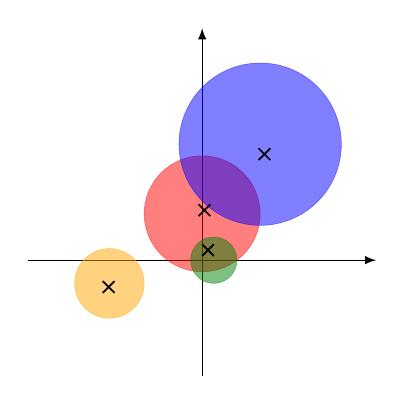
\begin{tikzpicture}

\definecolor{dimgray85}{RGB}{85,85,85}
\definecolor{gainsboro229}{RGB}{229,229,229}
\definecolor{green}{RGB}{0,128,0}
\definecolor{lightgray204}{RGB}{204,204,204}
\definecolor{orange}{RGB}{255,165,0}

\begin{axis}[
axis lines=middle,
inner axis line style={-latex},
grid=major,
width=6cm,
height=6cm,
xtick=\empty,
xmin=-15, xmax=15,
ytick=\empty,
ymin=-10, ymax=20,
]
\draw[draw=red,fill=red,opacity=0.5,very thin] (axis cs:0,4) circle (5);
\draw[draw=blue,fill=blue,opacity=0.5,very thin] (axis cs:5,10) circle (7);
\draw[draw=green,fill=green,opacity=0.5,very thin] (axis cs:1,0) circle (2);
\draw[draw=orange,fill=orange,opacity=0.5,very thin] (axis cs:-8,-2) circle (3);

\def\r{3}

%\addplot [semithick, red, mark=*, mark size=\r, mark options={solid}, only marks]
%table {%
%0 4
%};
%\addlegendentry{1\mi}
%\addplot [semithick, blue, mark=*, mark size=\r, mark options={solid}, only marks]
%table {%
%5 10
%};
%\addlegendentry{(5+10\mi)}
%\addplot [semithick, green, mark=*, mark size=\r, mark options={solid}, only marks]
%table {%
%1 0
%};
%\addlegendentry{(1)}
%\addplot [semithick, orange, mark=*, mark size=\r, mark options={solid}, only marks]
%table {%
%-8 -2
%};
%\addlegendentry{(-8-2j)}

\addplot [semithick, black, mark=x, mark size=\r, mark options={solid}, only marks, forget plot]
table {%
-8.06720901070025 -2.31297809243462
};
\addplot [semithick, black, mark=x, mark size=\r, mark options={solid}, only marks, forget plot]
table {%
5.36805383956579 9.13980083948909
};
\addplot [semithick, black, mark=x, mark size=\r, mark options={solid}, only marks, forget plot]
table {%
0.195375871819944 4.3072164295875
};
\addplot [semithick, black, mark=x, mark size=\r, mark options={solid}, only marks, forget plot]
table {%
0.503779299314509 0.865960823358021
};
\end{axis}

\end{tikzpicture}
\end{marginfigure}

\begin{theo}
    Soit $A \in \M_n(\K)$. Alors, $$\Sp(A) \subset \bigcup\limits_{i=1}^{n} \overline{\mathscr{B}} \Bigg( a_{i,i}, \sum\limits_{k \not = i} |a_{i,k}| \Bigg).$$ \\
    Ces disques sont nommés les \href{https://fr.wikipedia.org/wiki/Théorème_de_Gerschgorin}{disques de \textsc{Gerschgorin}} (cf. thème \textit{Localisation des valeurs propres}, Ch. 11 \cite{acamanes}).
\end{theo}

\begin{preuve}
    Soit $\lambda \in \Sp(A)$. La matrice $A - \lambda \I_n$ n'est pas inversible donc n'est pas à DSD i.e. pour tout $i \in \llbracket 1, n \rrbracket$,
    $$|a_{i,i} - \lambda| \leqslant \sum_{k \not= i} |a_{i,k}|.$$
    Le spectre de la matrice $A$ est donc inclus dans la réunion des disques de centre $a_{i,i}$ et de rayon $\sum\limits_{k \not=i} a_{i,k}$.
\end{preuve}    

\begin{prop}
    Soit $A \in \M_n(\R)$ à DSD telle que $a_{i,i} > 0$ pour tout $i \in \llbracket 1, n \rrbracket$. Alors $\mathrm{det}(A) > 0$. 
\end{prop}

\begin{preuve}
        $\det(A) = \prod\limits_{\lambda \in \Sp(A)} \lambda$. Distinguer les vap complexes et réelles...
\end{preuve}


% \begin{marginfigure}
%        \input{disques_gerschgorin}
%    \end{marginfigure}

\section{Matrices stochastiques}
\marginnote[3cm]{
    $$
    \begin{pmatrix}
    1/2 & 1/2 & 0 \\
    3/4 & 1/8 & 1/8 \\
    0 & 1/3 & 2/3
    \end{pmatrix}
    $$
}

\begin{marginfigure}[5cm]
    \centering
    \resizebox{5.5cm}{5.5cm}{%
    \begin{tikzpicture}
        \node[state] (s1) {1};
        \node[state, below right of=s1] (s2) {2};
        \node[state, below left of=s1] (s3) {3};
    
        \draw (s1) edge[loop above] node {$1/2$} (s1);
        \draw (s1) edge[bend left] node {$1/2$} (s2);
        %\draw (s1) edge[bend right, above left] node {0} (s3);
    
        \draw (s2) edge[bend left, above right] node {$3/4$} (s1);
        \draw (s2) edge[loop right] node {$1/8$} (s2);
        \draw (s2) edge[bend right] node {$1/8$} (s3);
    
        %\draw (s3) edge[bend right] node {0} (s1);
        \draw (s3) edge[bend right] node {$1/3$} (s2);
        \draw (s3) edge[loop left] node {$2/3$} (s3);
    \end{tikzpicture}    
}

  %  \begin{tikzpicture}
  %      \node[state] (s1) {État 1};
  %      \node[state, below right of=s1] (s2) {État 2};
   %     \node[state, below left of=s1] (s3) {État 3};
 %  
 %       \draw (s1) edge[loop above] node {$p_{1,1}$} (s1);
%        \draw (s1) edge[bend left] node {$p_{1,2}$} (s2);
%        \draw (s1) edge[bend right, above left] node {$p_{1,3}$} (s3);
    
 %       \draw (s2) edge[bend left, above right] node {$p_{2,1}$} (s1);
%        \draw (s2) edge[loop right] node {$p_{2,2}$} (s2);
%        \draw (s2) edge[bend right] node {$p_{2,3}$} (s3);
    
%        \draw (s3) edge[bend right] node {$p_{3,1}$} (s1);
%        \draw (s3) edge[bend right] node {$p_{3,2}$} (s2);
%        \draw (s3) edge[loop left] node {$p_{3,3}$} (s3);
%    \end{tikzpicture}    
    \caption*{\centering Une chaîne de \textsc{Markov} et sa matrice de transition.}
\end{marginfigure}

\marginnote[0cm]{Texte de \cite{oraux_x_ens_2} p. 59}
Les matrices stochastiques interviennent en probibilités. Si $X$ et $Y$ sont deux variables aléatoires à valeurs dans $E \defeq \llbracket 1, k \rrbracket$, alors la matrice $A \defeq (a_{i,j}) \in \M_k(\R)$ définie par $a_{i,j} \defeq \P(Y = j | X = i)$ est stochastique, ce qui par définition signifie qu'on a $a_{i,j} \geqslant 0\ (1 \leqslant i, j \leqslant k)$ et $\sum\limits_{j=1}^k a_{i,j} = 1\ (1 \leqslant i \leqslant k)$. \\
L'évolution d'un système susceptible de prendre un nombre fini d'états notés $1, \dots, k$ est représentée mathématiquement par une suite $(X_n)_{n \geqslant 0}$ de variables aléatoires à valeurs dans $E$. C'est ce qu'on appelle un processus aléatoire (ou stochastique). Si $X_{n+1}$ s'obtient à partir de la valeur de $X_n$ et d'un tirage au sort effectué selon une loi ne dépendant que de cette valeur, on dit que le processus est une chaîne de \textsc{Markov}. Les exemples abondent: marches aléatoires, fortune d'un joueur, modélisation de l'alternance des voyelles et des consonnes dans un poème de \textsc{Pouchkine} (par \textsc{Markov} lui-même), ou prévision (en probabilité) des états  successifs d'un signal pour améliorer la compression en traitement du signal (\textsc{Shannon}) \\
Techniquement, on dit qu'une suite de variables aléatoires $(X_n)$ est une chaîne de \textsc{Markov} si \say{ la loi de l'état $n+1$ conditionnelle au passé de dépend que de l'état antérieur $n$ }, ce qui se traduit par
$$\P(X_{n+1}=j | X_0=i_0, \dots, X_n = i_n) = \P(X_{n+1} = j | X_n = i_n).$$
Si la matrice $A \defeq (a_{i,j}) \in \M_k(\R)$ définie par $a_{i,j} \defeq \P(Y = j | X = i)$ est indépendante de $n$, on dit que la chaîne de \textsc{Markov} est stationnaire. Si, dans ce dernier cas, on pose $Y_n \defeq \begin{pmatrix} \P(X_n = 1) \\ \vdots \\ \P(X_n = k) \end{pmatrix}$, pour tout $n \geqslant 0$, on obtient $Y_{n+1} = A Y_n$ et donc $Y_n = A^n Y_0$. \\
Le comportement (probabiliste) d'une chaîne de \textsc{Markov} stationnaire, et notamment son comportement asymptotique, est donc entièrement décrit par la donnée de la loi initiale $Y_0$ et des puissances de la matrice $A$. 

\begin{defi}
    Une matrice stochastique (matrice de transition d'une \nameref{chaîne_markov}) est une matrice $P \in \M_n([0, 1])$ telle que pour tout $i \in \llbracket 1, n \rrbracket, \sum\limits_{j=1}^{n} p_{i,j} = 1$. \\ Autrement dit, chaque ligne de $P$ est une vecteur de probabilité. \\
    On dit que $P$ est \emph{doublement stochastique} si $P$ et $\Trsp{P}$ sont stochastiques.
\end{defi}

\begin{exercice}
    \footnote{Exercice 5, TD 11} \\
    Soit $P$ une matrice stochastique.
    \begin{enumerate}
        \item Montrer que $1$ est valeur propre de $P$.
        \item Soit $v = \Trsp{(v_1 \cdots v_n)}$ un vecteur propre associé à la valeur propre $1$. En considérant $|v_{i_0}| = \max\limits_{1 \leqslant i \leqslant n} |v_i|$, montrer que le sous-espace propre associé à $E_1$ est de dimension $1$.
        \item Montrer que si $\lambda \in \C$ est une valeur propre de $P$, alors $| \lambda | \leqslant 1$.
        \item Soit $\lambda \in \C$ une valeur propre de $P$ telle que $|\lambda| = 1$ et $\title{x}$ un vecteur propre associé.
        \begin{enumerate}
            \item Montrer qu'il existe un vecteur propre associé à $\lambda$ tel que $\Ninf{x} = 1$. 
            \item Montrer qu'il existe $i_0 \in \llbracket 1, n \rrbracket$ tel que $\left| \sum\limits_{j=1}^n p_{i_0,j} x_j \right| = 1$.
            \item Soit $\theta$ l'argument principal de $\sum\limits_{j=1}^n p_{i_0,j} x_j$. Montrer que pour tout $j \in \llbracket 1, n \rrbracket, \Reel \left( \me^{-\mi \theta} x_j \right) = 1$.
            \item En déduire que $\lambda = 1$.
        \end{enumerate}
    \end{enumerate}
\end{exercice}

\begin{solution}
    L'objectif de l'exercice est de montrer que $\boxed{\Sp_{\C}(P) = \{1 \} }$.
    \begin{enumerate}
        \item 1 est valeur propre évidente de $P$ de vecteur propre associé $v = (1, \dots, 1)^\top$.
        \item Montrer que $\dim E_1 = 1$.
        \begin{itemize}
            \item Appliquer la même méthode que la démonstration du lemme d'\textsc{Hadamard}. \\
            Soit $X = \Trsp{(x_1, \dots, x_n)} \in E_1$. Montrons que $X \in \Vect(v)$. \\
            On montre que $|x_{i_0}| = \left| \sum\limits_{j=1}^{n} p_{i_0, j} x_j \right| = \sum\limits_{j=1}^{n} p_{i_0, j} |x_j|$ et on écrit $|x_{i_0}| = |x_{i_0}| \sum\limits_{j=1}^{n} p_{i_0, j}$. D'où, en faisant la différence, pour tout $j \in \llbracket 1, n \rrbracket,\ |x_{i_0}| = |x_j|$. De plus d'après la première relation, il y égalité dans l'inégalité triangulaire et donc les $v_j$ sont \emph{positivement liées}. Finalement, pour tout $j \in \llbracket1, n \rrbracket,\ v_j = v_{i_0}$ soit $\dim E_1 = 1$.
        \end{itemize}
        \item Montrer que si $\lambda \in \C$ est une valeur propre de $P$, alors $|\lambda| \leqslant 1$. \\
        Poser $X = (x_1, \dots, x_n)^\top$ un vecteur propre associé et appliquer encore une fois la même méthode; poser $\displaystyle |x_{i_0}|= \max_{1 \leqslant i \leqslant n} |x_i|$, écrire en module la ligne $i_0$ de l'égalité $\lambda X = P X$, diviser par $|x_{i_0}|$ (qui est non nul d'après la question précédente) puis majorer par $1$. \\
            
        Pour les curieux, lire \cite{matrices} page 59. 
        
        \begin{prop}
            Le \nameref{rayon_spectral} stochastique est égal à $1$.
        \end{prop}
    
        \item Les questions suivantes (à détailler éventuellement) consiste encore au même jeu avec la ligne $i_0$ et les propriétés de matrices stochastiques. 
    \end{enumerate}
\end{solution}


\section{Exercice 10 TD 11}
Soit $f \in \mathscr{L}(\K^n)$.

\begin{enumerate}
    \item On suppose que $f$ est diagonalisable. Montrer que tout sous-espace de $\K^n$ stable par $f$ admet un supplémentaire stable par $f$.\\
    Soit $F$ un sev de $E$ stable par $f$.
    \begin{itemize}
        \item Posons $\boxed{g = f_{\vert F}}$ qui est diagonalisable car $f$ l'est par hypothèse. 
        \item Soit $\mathscr{B}_F$ une base de $F$ formée de vep de $g$. 
        \item Soit $\mathscr{B}'$ une base de $E$ formée de vep de $f$ (qui existe car $f$ est diagonalisable).
        \item On \textbf{complète} $\mathscr{B}_F$ est une base $\mathscr{B}$ de E en prenant des vep $(\varepsilon_1, \cdots, \varepsilon_r)$ de $\mathscr{B}'$. On note $(\lambda_1, \dots, \lambda_r)$ les valeurs propres associées. 
        \item On pose G = $\mathrm{Vect}(\varepsilon_1, \dots, \varepsilon_r)$. De cette manière, $F$ et $G$ sont supplémentaires. Montrons que $G$ est stable par $f$. \\
        Soit $x = \sum\limits_{i=1}^{r} \mu_i \varepsilon_i \in G$. Donc $f(x) = \sum\limits_{i=1}^{r} \mu_i f(\varepsilon_i) =  \sum\limits_{i=1}^{r} \mu_i \lambda_i \varepsilon_i \in G$ et $G$ est stable par $f$.
    \end{itemize}
    
    \item Que dire de la réciproque dans $\C$ ? \\
    Montrons que $f$ est diagonalisable. On va montrer que $E = \bigoplus\limits_{\lambda \in \Sp(f)} E_\lambda (f)$.
    
    \begin{enumerate}
        \item \underline{Somme directe:} \\
        On pose $F = \bigoplus\limits_{\lambda \in \Sp(f)} E_\lambda (f)$ et $\Sp(f) = (\lambda_1, \dots, \lambda_r)$. \\
        Soit $x = \sum\limits_{i=1}^{r} x_i \in F$ où $x_i \in E_{\lambda_i}(f)$. Alors $f(x) = \sum\limits_{i=1}^{r} \underbrace{\lambda_i x_i}_{\in E_{\lambda_i}(f)} \in F$. Donc $F$ est stable par $f$.
        \item Montrons que $F = E$. \\
        Par hypothèse, $F$ admet un supplémentaire $G$ dans $\C^n$, stable par $f$. Montrons que $\boxed{G = \{0\}}$ en raisonnant par l'absurde. \\
        On pose $\boxed{g = f_{\vert F}}$. D'après le \textbf{théorème de \textsc{D'Alembert-Gauss}} sur $\C$, $g$ admet au moins une valeur propre $\mu \in \C$ de vep associé $x_\mu$. On montre que $x_\mu \in F \cap G$. Or $F$ et $G$ sont supplémentaires donc $x_\mu = 0_E$: contradiction. D'où le résultat. 
    \end{enumerate}
    \item Décrire un contre-exemple à la réciproque dans $\R$, en dimension 2. \\
    Considérer $R_\theta$. \textcolor{green}{à revoir}
\end{enumerate}

\section{Autour du commutant}
\begin{defi}[Commutant d'une matrice]
    Soient $A \in \M_n(\R)$ et $C(A) \defeq \ens[\big]{M \in \M_n(\R) \tq MA = AM }$.
\end{defi}

\begin{exercice}
    \source{\cite{exos_oraux} p. 119}
    Soit $E$ un $\K$-espace vectoriel de dimension finie et $u \in \Endo(E)$. Démontrer que $C(u)$ a une structure de $\K$-espace vectoriel puis que, si $u$ est diagonalisable:
    $$\dim C(u) = \smashoperator{\sum_{\lambda \in \Sp(u)}} \dim^2 E_\lambda(u).$$
\end{exercice}

\begin{solution}
    
\end{solution}

\begin{exercice}
    \source{\cite{acamanes} \href{https://acamanes.github.io/psi/psi_doc/exos_e11.pdf}{(Exercice 12 TD 11)}}
    Soit $A \in \M_n(\R)$.
    \begin{enumerate}
        \item 
        \begin{enumerate}
            \item Montrer que $C(A)$ est un sous-espace vectoriel de $\M_n(\R)$ stable par multiplication.
            \item Montrer que si $M \in C(A)$ et $M$ est inversible, alors $\Inv{M} \in C(A)$.
        \end{enumerate}
        \item Soit $D$ une matrice diagonale dont les coefficients diagonaux sont deux à deux distincts.
        \begin{enumerate}
            \item Déterminer $C(D)$.
            \item Montrer que $\big(\I_n, D, \dots, D^{n-1}\big)$ est une base de $C(D)$.
        \end{enumerate}
        \item On se limite au cas $n=2$.
        \begin{enumerate}
            \item Déterminer les matrices $A$ telles que $\dim C(A) = 4$.
            \item Montrer que $\dim C(A) \geqslant 2$. 
            \item On suppose que $\dim C(A) \geqslant 3$. En utilisant $F \defeq \Vect \big\{ \mathrm{E}_{1, 1}, \mathrm{E}_{1, 2} \big\}$ ou $G \defeq \Vect \big\{ \mathrm{E}_{2, 1}, \mathrm{E}_{2, 2} \big\}$, montrer que $A = \lambda \I_2$.
            \item Pour tout $A \in \M_2(\R)$, déterminer une base de $C(A)$.
        \end{enumerate}
    \end{enumerate}
\end{exercice}

\begin{enumerate}
    \item \emph{Montrer que C(A) est un sous-espace vectoriel de $\M_n(\R)$.} \\
    Au lieu de redémontrer les propriétés d'un sev, on peut voir $C(A)$ comme le \textbf{noyau de l'application linéaire} $M \mapsto MA - AM$ ce qui donne directement le résultat. 
    \item On veut montrer que $M^{-1} A = A M^{-1}$ i.e. $A = M A M^{-1}$ ce qui est vrai car $M A = A M$.
    \item
    \begin{itemize}
        \item $C(D) = \mathscr{D}_n$ (l'ensemble des matrices diagonales de taille $n$) \textcolor{red}{(ne pas oublier de montrer la double inclusion)}.
        \item Comme $| \mathscr{B} | = \dim C(D)$, il suffit de montrer la liberté de $\mathscr{B}$. \\
        Soit $(\lambda_0, \dots, \lambda_{n-1}) \in \R^n$ tel que $\sum\limits_{k=0}^{n-1} \lambda_k D^k = 0_n$. \\
        \textcolor{green}{Revoir le caractère générateur avec les polynômes d'interpolation.}
        \begin{itemize}
            \item Pour tout $i \in \llbracket 1, n \rrbracket$, $\sum\limits_{k=0}^{n-1} \lambda_k d_i = 0_n \quad (*)$. Donc le polynôme $P = \sum\limits_{k=0}^{n-1} \lambda_k X^k$ qui est de dégré $n-1$ et prossède $n$ racines distinctes et est donc le polynôme nul. On en déduit que les $\lambda_i$ sont tous nuls. La famille $\mathscr{B}$ est bien libre et forme une base de $C(D)$.
            \item Les relations $(*)$ forment un système de \nom{Vandermonde} de $n$ équations à $n$ inconnues. Comme les coefficients $d_i$ sont deux à deux distincts, le système est inversible et son unique solution est le vecteur colonne nul.
        \end{itemize}
    \end{itemize}
    \item On se limite au cas $n = 2$. 
    \begin{enumerate}
        \item Déterminer les matrices $A$ telles que $\dim C(A) = 4$. \\
        $C(A) = \M_2(\R)$ car $C(A) \subset \M_2(\R)$ et il y égalité des dimensions. \\
        \ptnclegras{Évaluer les commutant en les matrices de la base canoniques de $\M_2(\R)$}: on trouve que A est scalaire. \\
        \textcolor{red}{Ne pas oublier de montrer la réciproque}. 
        \item Montrer que $\dim C(A) \geqslant 2$. \\
        Si $A$ est scalaire, cf. question précédente. \\
        Sinon montrer que la famille $\big\{ \I_2, A \big\} \subset C(A)$ est libre. 
        \item Enoncé... \\
    \end{enumerate}
\end{enumerate}

\section{Que dire si \texorpdfstring{$u \circ u$}{u^2} est diagonalisable ?}
\input{chapitres/reduction_des_endomorphismes/que_dire_si_u_carre_est_diagonalisable}

\section{Spectre de \texorpdfstring{$\Id_E-uv$ et $\Id_E-vu$}{IdE-uv et IdE - vu}} \label{spectre_I-uv_et_I-vu}
\begin{exercice}
    \marginnote[0cm]{\cite{exos_oraux}}
    Soient $u$ et $v$ deux endomorphismes d'un espace $E$ de dimension finie $n \in \Ne$. Prouver que $\Id_E - uv$ et $\Id_E - vu$ ont les mêmes valeurs propres. \\
    En déduire que $\Id_E - uv$ est inversible si $\Id_E - vu$ l'est aussi, relier les inverses.
\end{exercice}

Soient $u$ et $v$ deux endomorphismes d'un espace $E$ de dimension $n$.

\begin{enumerate}
    \item Montrer que $\Id_E-uv$ et $\Id_E-vu$ ont les mêmes valeurs propres.
    \begin{itemize}
        \item Montrer que ces deux endomorphismes ont même polynôme caractéristique en posant les deux matrices
        $$
        A = 
        \begin{pmatrix}
            U & \lambda \I_n \\
            \I_n & V
        \end{pmatrix}
        \text{ et }
        B = 
        \begin{pmatrix}
            V & -\lambda \I_n \\
            -\I_n & 0_n
        \end{pmatrix}.
        $$
        \begin{align*}
            \det(AB) &= \det(BA) \\
            (-\lambda)^n \det(AB - \lambda \I_n) &= (-\lambda)^n \det(BA - \lambda \I_n)
        \end{align*}
    \end{itemize}
    \item En déduire que $\Id_E-uv$ est inversible si et seulement si $\Id_E-vu$ l'est, relier les inverses. 
    \begin{itemize}
        \item $f \in \Gl(E) \Longleftrightarrow 0 \not \in \Sp(f)$
        \item Évaluer le résultat précédent en $\lambda = 1$.
        \item Analogie avec l'inversion par sommation géométrique des endomorphismes nilpotents (cf. \nameref{indice_nilpotence})
    \end{itemize}
\end{enumerate}

\section{Raciné carrée d'une matrice}
\url{https://share.miple.co/content/CtwFAB5leFp4M}

\begin{box_titre}{DS6}
    On note $\mathrm{Rac}(A) = \{ R \in \M_n(\R),\ R^2 = A \}$. \\
    $\blacktriangleright$ Soit $A \in \M_n(\R)$. $\mathrm{Rac}(A)$ est une partie fermée de $\M_n(\R)$. \\
    $\blacktriangleright$ $\mathrm{Rac}(\I_n)$ n'est pas une partie bornée de $\M_n(\R)$ pour $n \geqslant 3$. 
\end{box_titre}

\begin{box_titre}{Racine carrée de matrices symétriques positives}
    Pour tout $A \in \mathscr{S}^+(\R)$, il existe une unique matrice $B \in \mathscr{S}^+(\R)$ telle que $A = B^2$. 
\end{box_titre}

\underline{Exercice 11, TD 11:}\\
Soit $A = 
\begin{pmatrix}
    -1 & 2 & 3 \\
    0 & - 1 & 4 \\
    0 & 0 & 1
\end{pmatrix}. 
$ Montrer que $A$ n'a pas de racine dans $\M_3(\R)$. 

\section{Réduction d'une matrice creuse}
\begin{tcolorbox}
    Soit $n \geqslant 2$. On pose:
    $$
    A = 
        \begin{pmatrix}
              &        &   & c \\
              &  (0)   &   & \vdots \\
              &        &   & c \\
            b & \cdots & b & a
        \end{pmatrix}
        \in \M_n(\R).
    $$
    Étudier la possibilité de diagonaliser $A$ sur $\R$.
\end{tcolorbox}

\underline{Remarques:}\\
$\blacktriangleright$ Si $b = c$ alors $A$ est symétrique réelle donc diagonalisable. \\
$\blacktriangleright$ $A$ est au plus de rang 2. Donc par le \textbf{théorème du rang}, 0 est une valeur propre de $A$ de multiplicité au moins $n-2$.

\section{Vecteurs propres de $\Trsp{\com(A)}$}
\begin{exercice}
    Soit $A \in \M_n(\K)$. Montrer que 
    $$\Sp(A) \subset \Sp \big( \Trsp{\com(A)} \big).$$
\end{exercice}
\marginnote[0cm]{
    $$A \times\ \Trsp{\com(A)} = \Trsp{\com(A)} \times A = \det(A) \I_n$$
}
\begin{elem_sol}
    Soit $\lambda \in \Sp(A)$ et $X$ un vecteur propre associé. Alors $\lambda (BX) = \det(A) X$. 
        
    \begin{itemize}
        \item $\lambda \not = 0$: $BX = \frac{\det(A)}{\lambda}X$. 
        \item $\lambda = 0$: alors $\det(A) = 0$ et $\Rg(A) \leqslant n-1$. 
        \begin{itemize}
            \item $\Rg(A) \leqslant n-2$: supposer par l'absurde qu'il existe un déterminant mineur de $A$ non nul. 
            \item $\Rg(A) = n-1$: $X \in \Ker(A)$ qui est une droite vectorielle. 
            $$A \text{ et } B \text{ commutent donc } \Ker(A) \text{ est stable par } B$$
        \end{itemize}
    \end{itemize}
\end{elem_sol}


\section{Éléments propres de $MN$, de $NM$}
\begin{prop}{}
    Soient $M$ et $N$ dans $\M_n(\K)$.
    \begin{itemize}
        \item $$0 \in \Sp(MN) \iff 0 \in \Sp(NM)$$
        \item Soit $\lambda \in \Ke$,
        $$\dim E_\lambda(MN) = \dim E_\lambda(NM)$$
    \end{itemize}
\end{prop}

Soit $M, N \in \M_n(\K)$. 
\begin{enumerate}
    \item ...
    \item \emph{Soit $\lambda \in \Ke$, montrer que $\dim(E_\lambda (MN)) = \dim(E_\lambda (NM))$.} \\
    On remarque que si $X \in E_\lambda (MN)$ alors $NX \in E_\lambda (NM)$. On pose alors:
    $$
        \fonction[\varphi]{E_\lambda (MN)}{E_\lambda (NM)}{X}{NX}.
    $$
    On montre que $\varphi$ est injective et on en déduit que $\dim(E_\lambda (MN)) \leqslant \dim(E_\lambda (NM))$. Par symétrie des rôles de $M$ et de $N$, on montre l'inégalité dans le sens inverse et on en déduit l'égalité.
    \item ...
    \item ...
\end{enumerate}


\section{Diagonalisation ou trigonalisation simultanée}
\begin{box_titre}{Endomorphismes codiagonalisables}
    Soit $E$ un espace vectoriel de dimension finie. Soient $u$ et $v$ deux endomorphismes de $E$ diagonalisables. \\
    On dit que $u$ et $v$ sont \emph{codiagonalisables} s'il existe une base $\mathscr{B}$ de $E$ telle que $\mathrm{Mat}_\mathscr{B}(u)$ et $\mathrm{Mat}_\mathscr{B}(v)$ sont diagonalisables. 
    $$u, v \text{ sont codiagonalisables } \Longleftrightarrow u, v \text{ commutent}.$$
\end{box_titre}

\begin{itemize}
    \item $(\Leftarrow)$ Indication: si $D$ et $\widetilde{D}$ sont diagonales, alors $D \times \widetilde{D} = \widetilde{D} \times D$.
    \item $(\Rightarrow)$ Notons $\mathrm{Sp}(u) = \{ \lambda_i,\ i \in \llbracket1, p \rrbracket \}$. Comme $u$ est diagonalisable, alors $E = \bigoplus\limits_{i = 1}^{p} E_{\lambda_i}(u)$. \\
    Soit $i \in \llbracket 1, p \rrbracket$. Comme $v$ commute avec $u - \lambda_i \mathrm{Id}_E$, $\boxed{E_{\lambda_i}(u) \text{ est stable par } v}$. \\
    En notant $\boxed{v_i \text{ l'endomorphisme induit par } v \text{ sur } E_{\lambda_i}(u)}$, comme $v$ est diagonalisable, $\boxed{v_i \text{ est diagonalisable}}$. Ainsi, il existe $(e_{i, 1}, \dots, e_{i, r_i})$ une base de $E_{\lambda_i}(u)$ formée de vecteurs propres de $v_i$. De plus, $e_{i, j}$ est un vecteur propre de $u$. \\
    Finalement, $\boxed{(e_{i, 1}, \dots, e_{i, r_i})_{1 \leqslant i \leqslant p}}$ est une base de $E$ constituée de vecteurs propres de $u$ et de $v$. Ainsi, $u$ et $v$ sont diagonalisables dans cette même base. 
\end{itemize}

\marginnote[-10cm]{
    \begin{kaobox}[frametitle=Décomposition de $E$ en somme de sous-espaces stables supplémentaire]
        Si $E$ est de dimension finie non nulle et $\chi_f = \prod\limits_{i=1}^{k}(f-\lambda_i)^{\alpha_i}$, alors
        $$E = \bigoplus_{i=1}^{k} \Ker(f-\lambda_i \Id_E)^{\alpha_i}.$$
        \begin{itemize}
            \item Les $\Ker(f-\lambda_i \Id_E)^{\alpha_i}$ sont supplémentaires et stables par $f$. Donc, dans tout base adaptée à cette décomposition, la matrice de $f$ est diagonale par blocs. 
            \item La restriction de $f$ à $\Ker(f-\lambda_i)^{\alpha_i}$ induit un endomorphisme $f_i$ de ce sous-espace. $f_i$ admet une et une seule valeur propre à savoir $\lambda_i$ et $f_i - \lambda_i \Id_{\Ker(f-\lambda_i)^{\alpha_i}}$ est nilpotente d'indice inférieur ou égal à $\alpha_i$. 
        \end{itemize}
    \end{kaobox}
    Source: fiche de \cite{maths-france}.
}

A rajouter:
\begin{itemize}
    \item Matrices dont le spectre est un singleton
    \item Réduction simultanée
    \item Endomorphismes symétriques à valeurs propres positives
    \item Matrices de rang 1
    \item Critère de non-diagonalisabilité sur $\C$
    \item Commutant d'un endomorphisme diagonalisable 
    \item Déterminant, réduction d'une matrice tridiagonale 
\end{itemize}